% Options for packages loaded elsewhere
\PassOptionsToPackage{unicode}{hyperref}
\PassOptionsToPackage{hyphens}{url}
%
\documentclass[
]{article}
\usepackage{amsmath,amssymb}
\usepackage{iftex}
\ifPDFTeX
  \usepackage[T1]{fontenc}
  \usepackage[utf8]{inputenc}
  \usepackage{textcomp} % provide euro and other symbols
\else % if luatex or xetex
  \usepackage{unicode-math} % this also loads fontspec
  \defaultfontfeatures{Scale=MatchLowercase}
  \defaultfontfeatures[\rmfamily]{Ligatures=TeX,Scale=1}
\fi
\usepackage{lmodern}
\ifPDFTeX\else
  % xetex/luatex font selection
\fi
% Use upquote if available, for straight quotes in verbatim environments
\IfFileExists{upquote.sty}{\usepackage{upquote}}{}
\IfFileExists{microtype.sty}{% use microtype if available
  \usepackage[]{microtype}
  \UseMicrotypeSet[protrusion]{basicmath} % disable protrusion for tt fonts
}{}
\makeatletter
\@ifundefined{KOMAClassName}{% if non-KOMA class
  \IfFileExists{parskip.sty}{%
    \usepackage{parskip}
  }{% else
    \setlength{\parindent}{0pt}
    \setlength{\parskip}{6pt plus 2pt minus 1pt}}
}{% if KOMA class
  \KOMAoptions{parskip=half}}
\makeatother
\usepackage{xcolor}
\usepackage[margin=1in]{geometry}
\usepackage{color}
\usepackage{fancyvrb}
\newcommand{\VerbBar}{|}
\newcommand{\VERB}{\Verb[commandchars=\\\{\}]}
\DefineVerbatimEnvironment{Highlighting}{Verbatim}{commandchars=\\\{\}}
% Add ',fontsize=\small' for more characters per line
\usepackage{framed}
\definecolor{shadecolor}{RGB}{248,248,248}
\newenvironment{Shaded}{\begin{snugshade}}{\end{snugshade}}
\newcommand{\AlertTok}[1]{\textcolor[rgb]{0.94,0.16,0.16}{#1}}
\newcommand{\AnnotationTok}[1]{\textcolor[rgb]{0.56,0.35,0.01}{\textbf{\textit{#1}}}}
\newcommand{\AttributeTok}[1]{\textcolor[rgb]{0.13,0.29,0.53}{#1}}
\newcommand{\BaseNTok}[1]{\textcolor[rgb]{0.00,0.00,0.81}{#1}}
\newcommand{\BuiltInTok}[1]{#1}
\newcommand{\CharTok}[1]{\textcolor[rgb]{0.31,0.60,0.02}{#1}}
\newcommand{\CommentTok}[1]{\textcolor[rgb]{0.56,0.35,0.01}{\textit{#1}}}
\newcommand{\CommentVarTok}[1]{\textcolor[rgb]{0.56,0.35,0.01}{\textbf{\textit{#1}}}}
\newcommand{\ConstantTok}[1]{\textcolor[rgb]{0.56,0.35,0.01}{#1}}
\newcommand{\ControlFlowTok}[1]{\textcolor[rgb]{0.13,0.29,0.53}{\textbf{#1}}}
\newcommand{\DataTypeTok}[1]{\textcolor[rgb]{0.13,0.29,0.53}{#1}}
\newcommand{\DecValTok}[1]{\textcolor[rgb]{0.00,0.00,0.81}{#1}}
\newcommand{\DocumentationTok}[1]{\textcolor[rgb]{0.56,0.35,0.01}{\textbf{\textit{#1}}}}
\newcommand{\ErrorTok}[1]{\textcolor[rgb]{0.64,0.00,0.00}{\textbf{#1}}}
\newcommand{\ExtensionTok}[1]{#1}
\newcommand{\FloatTok}[1]{\textcolor[rgb]{0.00,0.00,0.81}{#1}}
\newcommand{\FunctionTok}[1]{\textcolor[rgb]{0.13,0.29,0.53}{\textbf{#1}}}
\newcommand{\ImportTok}[1]{#1}
\newcommand{\InformationTok}[1]{\textcolor[rgb]{0.56,0.35,0.01}{\textbf{\textit{#1}}}}
\newcommand{\KeywordTok}[1]{\textcolor[rgb]{0.13,0.29,0.53}{\textbf{#1}}}
\newcommand{\NormalTok}[1]{#1}
\newcommand{\OperatorTok}[1]{\textcolor[rgb]{0.81,0.36,0.00}{\textbf{#1}}}
\newcommand{\OtherTok}[1]{\textcolor[rgb]{0.56,0.35,0.01}{#1}}
\newcommand{\PreprocessorTok}[1]{\textcolor[rgb]{0.56,0.35,0.01}{\textit{#1}}}
\newcommand{\RegionMarkerTok}[1]{#1}
\newcommand{\SpecialCharTok}[1]{\textcolor[rgb]{0.81,0.36,0.00}{\textbf{#1}}}
\newcommand{\SpecialStringTok}[1]{\textcolor[rgb]{0.31,0.60,0.02}{#1}}
\newcommand{\StringTok}[1]{\textcolor[rgb]{0.31,0.60,0.02}{#1}}
\newcommand{\VariableTok}[1]{\textcolor[rgb]{0.00,0.00,0.00}{#1}}
\newcommand{\VerbatimStringTok}[1]{\textcolor[rgb]{0.31,0.60,0.02}{#1}}
\newcommand{\WarningTok}[1]{\textcolor[rgb]{0.56,0.35,0.01}{\textbf{\textit{#1}}}}
\usepackage{longtable,booktabs,array}
\usepackage{calc} % for calculating minipage widths
% Correct order of tables after \paragraph or \subparagraph
\usepackage{etoolbox}
\makeatletter
\patchcmd\longtable{\par}{\if@noskipsec\mbox{}\fi\par}{}{}
\makeatother
% Allow footnotes in longtable head/foot
\IfFileExists{footnotehyper.sty}{\usepackage{footnotehyper}}{\usepackage{footnote}}
\makesavenoteenv{longtable}
\usepackage{graphicx}
\makeatletter
\def\maxwidth{\ifdim\Gin@nat@width>\linewidth\linewidth\else\Gin@nat@width\fi}
\def\maxheight{\ifdim\Gin@nat@height>\textheight\textheight\else\Gin@nat@height\fi}
\makeatother
% Scale images if necessary, so that they will not overflow the page
% margins by default, and it is still possible to overwrite the defaults
% using explicit options in \includegraphics[width, height, ...]{}
\setkeys{Gin}{width=\maxwidth,height=\maxheight,keepaspectratio}
% Set default figure placement to htbp
\makeatletter
\def\fps@figure{htbp}
\makeatother
\setlength{\emergencystretch}{3em} % prevent overfull lines
\providecommand{\tightlist}{%
  \setlength{\itemsep}{0pt}\setlength{\parskip}{0pt}}
\setcounter{secnumdepth}{5}
\usepackage[spanish]{babel}
\usepackage{fontspec}
\ifLuaTeX
  \usepackage{selnolig}  % disable illegal ligatures
\fi
\IfFileExists{bookmark.sty}{\usepackage{bookmark}}{\usepackage{hyperref}}
\IfFileExists{xurl.sty}{\usepackage{xurl}}{} % add URL line breaks if available
\urlstyle{same}
\hypersetup{
  pdftitle={Tarea 1},
  pdfauthor={José Ignacio Rojas Zárate, C16911; Montserrat Beirute Abarca, C10997; Valeria Vásquez Venegas, C18373},
  hidelinks,
  pdfcreator={LaTeX via pandoc}}

\title{Tarea 1}
\usepackage{etoolbox}
\makeatletter
\providecommand{\subtitle}[1]{% add subtitle to \maketitle
  \apptocmd{\@title}{\par {\large #1 \par}}{}{}
}
\makeatother
\subtitle{Estadística Actuarial II}
\author{José Ignacio Rojas Zárate, C16911 \and Montserrat Beirute
Abarca, C10997 \and Valeria Vásquez Venegas, C18373}
\date{17 de enero de 2024}

\begin{document}
\maketitle

{
\setcounter{tocdepth}{2}
\tableofcontents
}
\newpage

\hypertarget{introducciuxf3n}{%
\section{Introducción}\label{introducciuxf3n}}

El presente documento prestan el código y resultados a los ejercicios de
la Tarea 1 del curso. Para su realización, se utilizó el programa R
studio.

Este trabajo requirió de los siguientes paquetes:

\begin{Shaded}
\begin{Highlighting}[]
\CommentTok{\#{-}{-}{-}Paquetes{-}{-}{-}{-}{-}{-}{-}{-}{-}{-}{-}{-}{-}{-}{-}{-}{-}{-}{-}{-}{-}{-}{-}{-}{-}{-}{-}{-}{-}{-}{-}{-}{-}{-}{-}{-}{-}{-}{-}{-}{-}{-}{-}{-}{-}{-}}

\FunctionTok{library}\NormalTok{(stringr) }\CommentTok{\# para cambiar todas las commas a puntos en la columna Ultimo Salario}
\FunctionTok{library}\NormalTok{(ggplot2) }\CommentTok{\# para hacer los gráficos}
\FunctionTok{library}\NormalTok{(univariateML) }\CommentTok{\# para hacer el análisis AIC}
\FunctionTok{library}\NormalTok{(rriskDistributions) }\CommentTok{\# para hacer el análisis AIC}
\FunctionTok{library}\NormalTok{(boot) }\CommentTok{\# para hacer el bootstrap}
\FunctionTok{library}\NormalTok{(ks) }\CommentTok{\# para Kernel smoothing}
\FunctionTok{library}\NormalTok{(knitr) }\CommentTok{\# para presentar mejor los datos en formato tabla}
\FunctionTok{options}\NormalTok{(}\AttributeTok{scipen =} \DecValTok{999}\NormalTok{) }\CommentTok{\# para no utilizar notación científica}
\FunctionTok{library}\NormalTok{(cowplot) }\CommentTok{\# para hacer graficos más atractivos}
\end{Highlighting}
\end{Shaded}

El presente trabajo utilizó la base de datos ``BaseSalarios'' brindada
por el profesor Esteban Bermúdez Aguilar. A continuación se presenta el
código para la lectura de la base de datos, así como también unos
ajustes para poder manipular y extraer la información de los datos.

\begin{Shaded}
\begin{Highlighting}[]
\CommentTok{\#{-}{-}{-}CSV y formatos{-}{-}{-}{-}{-}{-}{-}{-}{-}{-}{-}{-}{-}{-}{-}{-}{-}{-}{-}{-}{-}{-}{-}{-}{-}{-}{-}{-}{-}{-}{-}{-}{-}{-}{-}{-}{-}{-}{-}{-}{-}}

\CommentTok{\# Abrir y dar formato a la base de datos}

\NormalTok{base\_salarios }\OtherTok{\textless{}{-}} \FunctionTok{read.csv}\NormalTok{(}\StringTok{"BaseSalarios.csv"}\NormalTok{,  }\AttributeTok{sep =} \StringTok{";"}\NormalTok{)}

\NormalTok{base\_salarios}\SpecialCharTok{$}\NormalTok{Fec.Nac }\OtherTok{\textless{}{-}} \FunctionTok{as.Date}\NormalTok{(base\_salarios}\SpecialCharTok{$}\NormalTok{Fec.Nac, }\AttributeTok{format =} \StringTok{"\%d/\%m/\%Y"}\NormalTok{)}

\FunctionTok{colnames}\NormalTok{(base\_salarios)[}\DecValTok{5}\NormalTok{] }\OtherTok{=}\StringTok{"Ultimo.Salario"}

\NormalTok{base\_salarios }\OtherTok{\textless{}{-}} \FunctionTok{subset}\NormalTok{(base\_salarios, }\AttributeTok{select =} \SpecialCharTok{{-}}\NormalTok{X)}

\NormalTok{base\_salarios}\SpecialCharTok{$}\NormalTok{Ultimo.Salario }\OtherTok{\textless{}{-}} \FunctionTok{as.numeric}\NormalTok{(}\FunctionTok{str\_replace\_all}\NormalTok{(base\_salarios}\SpecialCharTok{$}\NormalTok{Ultimo.Salario, }\StringTok{","}\NormalTok{, }\StringTok{"."}\NormalTok{))}
\end{Highlighting}
\end{Shaded}

La base de datos tiene 5 columnas. A continuación, se presentan los
primeros seis registros de la base de datos ``BaseSalarios'' para poder
explicar la información de cada columna.

\begin{Shaded}
\begin{Highlighting}[]
\FunctionTok{kable}\NormalTok{(}\FunctionTok{head}\NormalTok{(base\_salarios\_temp), }\AttributeTok{caption =} \StringTok{"Primeros 6 registros de la base de datos"}\NormalTok{, }\AttributeTok{align =} \StringTok{"r"}\NormalTok{) }
\end{Highlighting}
\end{Shaded}

\begin{longtable}[]{@{}rrrrr@{}}
\caption{Primeros 6 registros de la base de datos}\tabularnewline
\toprule\noalign{}
ID & Fec.Nac & Sexo & Coutas & Ultimo.Salario \\
\midrule\noalign{}
\endfirsthead
\toprule\noalign{}
ID & Fec.Nac & Sexo & Coutas & Ultimo.Salario \\
\midrule\noalign{}
\endhead
\bottomrule\noalign{}
\endlastfoot
1 & 1945-01-30 & 1 & 323 & 2 784 093.18 \\
2 & 1949-06-17 & 2 & 342 & 532 324.93 \\
3 & 1951-04-19 & 2 & 13 & 225 517.69 \\
4 & 1950-02-05 & 2 & 323 & 1 612 733.09 \\
5 & 1952-02-06 & 2 & 185 & 1 411 502.30 \\
6 & 1954-01-10 & 2 & 284 & 1 915 751.19 \\
\end{longtable}

La columna \textbf{ID} cuenta el número de registros disponibles, en
este caso, se dispone de 106,002 registros. En la columna
\textbf{Fec.Nac} se encuentra la información de la fecha de nacimiento
de cada persona. En la tercera columna, \textbf{Sexo}, se observan los
números 1 y 2; específicamente, si el valor de Sexo es 1, corresponde a
hombres, y si es 2, corresponde a mujeres. La cuarta columna,
\textbf{Cuotas} indica la cantidad de cuotas que cada persona ha
aportado a un fondo de pensiones. Finalmente, la columna
\textbf{Ultimo.Salario} contiene el último salario reportado, expresado
en colones.

Es importante señalar que se tomó la decisión de eliminar dos registros
de la base de datos, ya que se consideraron datos atípicos, es decir,
outliers. Estos dos registros correspondían a salarios de 13 199 892 y
13 110 539 colones y estaban asociados a individuos del género
masculino. Ambos salarios superaban la media salarial de hombres en al
menos 11 953 340 colones.

\begin{Shaded}
\begin{Highlighting}[]
\NormalTok{base\_salarios }\OtherTok{\textless{}{-}}\NormalTok{ base\_salarios[}\SpecialCharTok{{-}}\DecValTok{84807}\NormalTok{, ] }\CommentTok{\# corresponde al salario 13 199 892}
\NormalTok{base\_salarios }\OtherTok{\textless{}{-}}\NormalTok{ base\_salarios[}\SpecialCharTok{{-}}\DecValTok{96367}\NormalTok{, ] }\CommentTok{\# corresponde al salario 13 110 539}
\end{Highlighting}
\end{Shaded}

\newpage

\hypertarget{parte-i}{%
\section{Parte I}\label{parte-i}}

\hypertarget{anuxe1lisis-descriptivo-de-las-variables-cuotas-y-salarios-con-respecto-a-la-variable-sexo}{%
\subsection{Análisis descriptivo de las variables Cuotas y Salarios con
respecto a la variable
Sexo}\label{anuxe1lisis-descriptivo-de-las-variables-cuotas-y-salarios-con-respecto-a-la-variable-sexo}}

De las 106,000 personas que contiene la base de datos utilizada, el
69.1\% son mujeres (73,279 mujeres). Por su parte, el 30.1\% restante
corresponde a hombres (32,721 hombres).

Es de interés conocer las diferencias o similitudes en los datos del
número de cuotas y los salarios según el sexo. Para ello, se presenta el
siguiente código:

\begin{Shaded}
\begin{Highlighting}[]
\NormalTok{resumen\_cuotas\_hombres }\OtherTok{\textless{}{-}}\FunctionTok{summary}\NormalTok{(base\_salarios}\SpecialCharTok{$}\NormalTok{Coutas[base\_salarios}\SpecialCharTok{$}\NormalTok{Sexo }\SpecialCharTok{==} \DecValTok{1}\NormalTok{])}

\NormalTok{varianza\_cuotas\_hombres }\OtherTok{\textless{}{-}} \FunctionTok{var}\NormalTok{(base\_salarios}\SpecialCharTok{$}\NormalTok{Coutas[base\_salarios}\SpecialCharTok{$}\NormalTok{Sexo }\SpecialCharTok{==} \DecValTok{1}\NormalTok{])}

\NormalTok{resumen\_cuotas\_hombres }\OtherTok{\textless{}{-}} \FunctionTok{c}\NormalTok{(resumen\_cuotas\_hombres, }\AttributeTok{Varianza =}\NormalTok{ varianza\_cuotas\_hombres)}

\NormalTok{resumen\_cuotas\_mujeres }\OtherTok{\textless{}{-}}\FunctionTok{summary}\NormalTok{(base\_salarios}\SpecialCharTok{$}\NormalTok{Coutas[base\_salarios}\SpecialCharTok{$}\NormalTok{Sexo }\SpecialCharTok{==} \DecValTok{2}\NormalTok{])}

\NormalTok{varianza\_cuotas\_mujeres }\OtherTok{\textless{}{-}} \FunctionTok{var}\NormalTok{(base\_salarios}\SpecialCharTok{$}\NormalTok{Coutas[base\_salarios}\SpecialCharTok{$}\NormalTok{Sexo }\SpecialCharTok{==} \DecValTok{2}\NormalTok{])}

\NormalTok{resumen\_cuotas\_mujeres }\OtherTok{\textless{}{-}} \FunctionTok{c}\NormalTok{(resumen\_cuotas\_mujeres, }\AttributeTok{Varianza =}\NormalTok{ varianza\_cuotas\_mujeres)}

\NormalTok{cuotas\_resumen }\OtherTok{\textless{}{-}} \FunctionTok{data.frame}\NormalTok{(}
  \AttributeTok{Estadistico =} \FunctionTok{c}\NormalTok{(}\StringTok{"Mínimo"}\NormalTok{, }\StringTok{"Primer cuartil (Q1)"}\NormalTok{, }\StringTok{"Mediana"}\NormalTok{, }\StringTok{"Promedio"}\NormalTok{, }\StringTok{"Tercer cuartil (Q3)"}\NormalTok{, }\StringTok{"Máximo"}\NormalTok{, }\StringTok{"Varianza"}\NormalTok{),}
  \AttributeTok{Hombres =} \FunctionTok{as.numeric}\NormalTok{(}\FunctionTok{round}\NormalTok{(resumen\_cuotas\_hombres,}\DecValTok{2}\NormalTok{)),}
  \AttributeTok{Mujeres =} \FunctionTok{as.numeric}\NormalTok{(}\FunctionTok{round}\NormalTok{(resumen\_cuotas\_mujeres,}\DecValTok{2}\NormalTok{))}
\NormalTok{)}
\end{Highlighting}
\end{Shaded}

A continuación, se presenta un cuadro con un resumen estadístico de los
datos del número de cuotas para hombres y mujeres.

\begin{longtable}[]{@{}lrr@{}}
\caption{Resumen estadístico de número de coutas por
sexo}\tabularnewline
\toprule\noalign{}
Estadistico & Hombres & Mujeres \\
\midrule\noalign{}
\endfirsthead
\toprule\noalign{}
Estadistico & Hombres & Mujeres \\
\midrule\noalign{}
\endhead
\bottomrule\noalign{}
\endlastfoot
Mínimo & 1.00 & 1.00 \\
Primer cuartil (Q1) & 61.00 & 66.00 \\
Mediana & 124.00 & 135.00 \\
Promedio & 135.19 & 142.97 \\
Tercer cuartil (Q3) & 198.00 & 213.00 \\
Máximo & 371.00 & 373.00 \\
Varianza & 7658.22 & 8187.47 \\
\end{longtable}

Como se puede observar, tanto para mujeres como para hombres, el número
mínimo de cuotas aportadas es tan solo una.

En general, y se va a justificar a continuación, se puede decir que las
mujeres en la base de datos han aportado más cuotas que los hombres.

Se puede notar que el 25\% de los hombres aportó 61 cuotas o menos,
mientras que en el caso de las mujeres, el 25\% aportó 66 cuotas o
menos.

Además, el 50\% de las mujeres aportó más de 135 cuotas, mientras que en
el caso de los hombres, fue de 124 cuotas.

El promedio de cuotas es más alto para las mujeres (142.97) que para los
hombres (135.19).

También, el 75\% de las mujeres aportó 213 cuotas o menos, mientras que
en el caso de los hombres, fue de 198 cuotas.

El valor máximo de cuotas aportadas para las mujeres fue de 373,
mientras que para los hombres fue de 371.

Es importante resaltar que para ambos sexos, la varianza indica que los
datos están alejados de la media y se presenta mucha variabilidad en los
datos de número de cuotas aportadas al fondo de pensiones.

Además, a continuación, se muestra el código y un cuadro con un resumen
estadístico de los datos del último salario reportado tanto para hombres
como para mujeres.

\begin{Shaded}
\begin{Highlighting}[]
\NormalTok{resumen\_salarios\_hombres }\OtherTok{\textless{}{-}}\FunctionTok{summary}\NormalTok{(base\_salarios}\SpecialCharTok{$}\NormalTok{Ultimo.Salario[base\_salarios}\SpecialCharTok{$}\NormalTok{Sexo }\SpecialCharTok{==} \DecValTok{1}\NormalTok{])}

\NormalTok{varianza\_salarios\_hombres }\OtherTok{\textless{}{-}} \FunctionTok{var}\NormalTok{(base\_salarios}\SpecialCharTok{$}\NormalTok{Ultimo.Salario[base\_salarios}\SpecialCharTok{$}\NormalTok{Sexo }\SpecialCharTok{==} \DecValTok{1}\NormalTok{])}

\NormalTok{resumen\_salarios\_hombres }\OtherTok{\textless{}{-}} \FunctionTok{c}\NormalTok{(resumen\_salarios\_hombres, }\AttributeTok{Varianza =}\NormalTok{ varianza\_salarios\_hombres)}

\NormalTok{resumen\_salarios\_mujeres }\OtherTok{\textless{}{-}}\FunctionTok{summary}\NormalTok{(base\_salarios}\SpecialCharTok{$}\NormalTok{Ultimo.Salario[base\_salarios}\SpecialCharTok{$}\NormalTok{Sexo }\SpecialCharTok{==} \DecValTok{2}\NormalTok{])}

\NormalTok{varianza\_salarios\_mujeres }\OtherTok{\textless{}{-}} \FunctionTok{var}\NormalTok{(base\_salarios}\SpecialCharTok{$}\NormalTok{Ultimo.Salario[base\_salarios}\SpecialCharTok{$}\NormalTok{Sexo }\SpecialCharTok{==} \DecValTok{2}\NormalTok{])}

\NormalTok{resumen\_salarios\_mujeres }\OtherTok{\textless{}{-}} \FunctionTok{c}\NormalTok{(resumen\_salarios\_mujeres, }\AttributeTok{Varianza =}\NormalTok{ varianza\_salarios\_mujeres)}

\NormalTok{salarios\_resumen }\OtherTok{\textless{}{-}} \FunctionTok{data.frame}\NormalTok{(}
  \AttributeTok{Estadistico =} \FunctionTok{c}\NormalTok{(}\StringTok{"Mínimo"}\NormalTok{, }\StringTok{"Primer cuartil (Q1)"}\NormalTok{, }\StringTok{"Mediana"}\NormalTok{, }\StringTok{"Promedio"}\NormalTok{, }\StringTok{"Tercer cuartil (Q3)"}\NormalTok{,}
                  \StringTok{"Máximo"}\NormalTok{, }\StringTok{"Varianza"}\NormalTok{),}
  \AttributeTok{Hombres =} \FunctionTok{format}\NormalTok{(}\FunctionTok{as.numeric}\NormalTok{(}\FunctionTok{round}\NormalTok{(resumen\_salarios\_hombres,}\DecValTok{2}\NormalTok{)),}\AttributeTok{big.mark =} \StringTok{" "}\NormalTok{),}
  \AttributeTok{Mujeres =} \FunctionTok{format}\NormalTok{(}\FunctionTok{as.numeric}\NormalTok{(}\FunctionTok{round}\NormalTok{(resumen\_salarios\_mujeres,}\DecValTok{2}\NormalTok{))}
\NormalTok{,}\AttributeTok{big.mark =} \StringTok{" "}\NormalTok{))}
\end{Highlighting}
\end{Shaded}

\begin{longtable}[]{@{}rrr@{}}
\caption{Resumen de Último Salario reportado por sexo}\tabularnewline
\toprule\noalign{}
Estadistico & Hombres & Mujeres \\
\midrule\noalign{}
\endfirsthead
\toprule\noalign{}
Estadistico & Hombres & Mujeres \\
\midrule\noalign{}
\endhead
\bottomrule\noalign{}
\endlastfoot
Mínimo & 10 880.92 & 10 223.99 \\
Primer cuartil (Q1) & 552 490.82 & 584 757.36 \\
Mediana & 1 104 956.42 & 1 062 461.32 \\
Promedio & 1 156 468.24 & 1 046 661.46 \\
Tercer cuartil (Q3) & 1 611 734.74 & 1 403 025.79 \\
Máximo & 8 154 905.08 & 7 290 150.00 \\
Varianza & 500 311 658 906.86 & 287 419 606 660.60 \\
\end{longtable}

En el Cuadro 3, se observa que el salario más bajo reportado le
pertenece a una mujer, siendo tan solo 656.93 colones menos que el
salario más bajo de los hombres.

En cuanto al Q1, se destaca que el 25\% de los hombres tuvieron un
último salario reportado de 552,491 colones o menos, mientras que el
25\% de las mujeres tuvieron un último salario de 584,757 colones o
menos. Es decir, en los últimos salarios más bajos, las mujeres
experimentaron ingresos superiores a los de los hombres.

Ahora en relación a la mediana, la mitad de los hombres ganó más de 1
104 956 colones, mientras que la mitad de las mujeres ganó menos (1 046
661 colones).

Además, el promedio de los últimos salarios fue mayor para los hombres,
aproximadamente 109 807 colones más alto.

Las diferencias se incrementan a medida que se consideran los últimos
salarios más altos. El 75\% de las mujeres ganaron 1 403 025.79 o menos,
mientras que el 75\% de los hombres ganaron 1 611 735 colones o menos.

El salario máximo reportado por hombres es 864 755 colones más alto que
el de las mujeres.

Es importante resaltar que la varianza para ambos sexos señala que los
datos están muy dispersos de la media, es decir hay una gran
variabilidad en los datos de último salario reportado.

\hypertarget{gruxe1fico-plotbox-para-el-salario-para-comparar-entre-las-categoruxedas-de-sexo}{%
\subsection{Gráfico plotbox para el salario para comparar entre las
categorías de
Sexo}\label{gruxe1fico-plotbox-para-el-salario-para-comparar-entre-las-categoruxedas-de-sexo}}

El siguiente gráfico plotbox permite tener una representación visual de
como se distribuyen los datos para cada sexo.

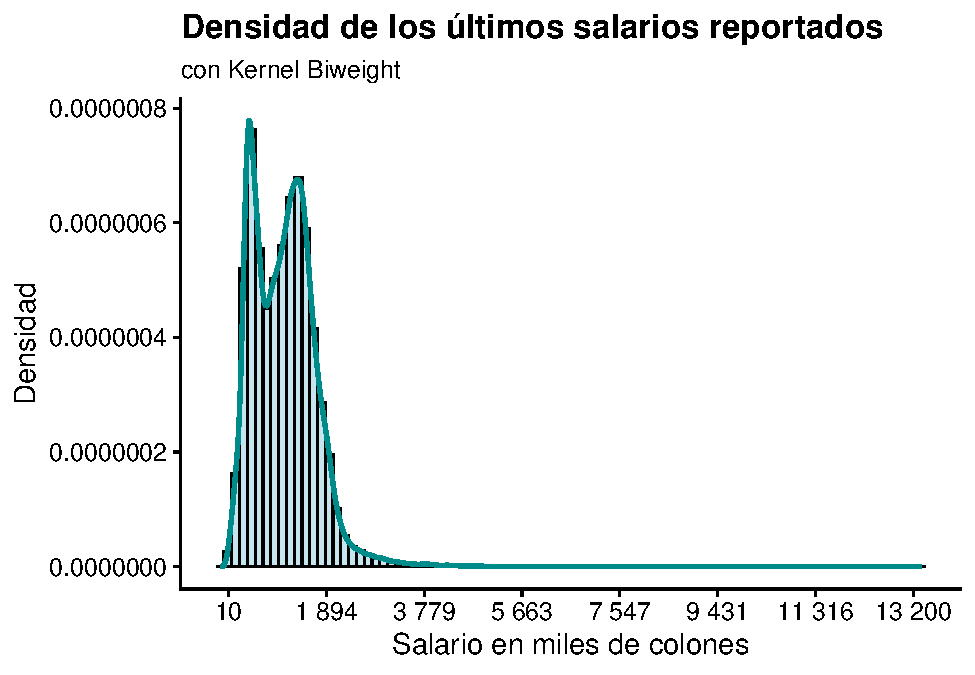
\includegraphics{Tarea1_files/figure-latex/unnamed-chunk-10-1.pdf}

Este gráfico destaca la presencia de salarios atípicos, identificados
como aquellos que están fuera de cada una de las cajas. Además, en este
gráfico, es de utilidad para visualizar el análisis presentado en la
sección anterior.

\hypertarget{conclusiones-con-respecto-a-los-salarios-y-sexo}{%
\subsection{Conclusiones con respecto a los salarios y
sexo}\label{conclusiones-con-respecto-a-los-salarios-y-sexo}}

Después de realizar el análisis descriptivo de los datos y para
complementar el gráfico anterior, se concluye que al dividir la
población por sexo, el 25\% de los hombres con los salarios más bajos
ganan menos que el 25\% de las mujeres con salarios más bajos. Sin
embargo, cuando se considera el 50\% de los hombres que ganan más, estos
perciben un salario mayor que el 50\% de las mujeres que ganan más. Esta
tendencia se evidencia claramente en el gráfico anterior, donde la parte
superior de la caja, que está por encima de la línea de la mediana, es
más amplia en el caso de los hombres.

Para respaldar este argumento, se observa que el promedio de los últimos
salarios fue mayor para los hombres, aproximadamente 109 807 colones más
alto que el de las mujeres.

No obstante, es importante señalar que la varianza de los salarios es
mayor para los hombres, y los valores atípicos en los salarios
masculinos también son más altos que los de las mujeres.

En este sentido, los salarios de los hombres parecen ser relativamente
más altos que los de las mujeres, aunque las diferencias no resultan
significativas. Ambos tienen personas con salarios más altos que la
mayoría.

\hypertarget{prueba-de-hipuxf3tesis-sobre-las-medias-de-las-categoruxedas-de-sexo}{%
\subsection{Prueba de hipótesis sobre las medias de las categorías de
sexo}\label{prueba-de-hipuxf3tesis-sobre-las-medias-de-las-categoruxedas-de-sexo}}

En relación a las medias, se cree que las medias de los salarios para
hombres y mujeres son diferentes. Para verificar lo expresado
anteriormente, se llevó a cabo la siguiente prueba de hipótesis.

En este caso, se llevó a cabo un \textbf{Welch Two Sample t-test}, la
cual es una prueba estadística que permite comparar las medias de dos
muestras. En este caso, el tamaño de las muestras y sus varianzas
difieren.

Para realizar una prueba de hipótesis se necesitan tres cosas: la
hipótesis nula (H0), el estadístico de prueba (t) y la distribución del
estadístico de prueba.

En este caso particular:

\begin{enumerate}
\def\labelenumi{\arabic{enumi}.}
\tightlist
\item
  H0: La diferencia entre la media de los últimos salarios de los
  hombres y la media de los últimos salarios de las mujeres es 0.
\item
  El estadístico de prueba es t, el cual se puede calcular de la
  siguiente manera:
  \[ t = \frac{\bar{X}_1 - \bar{X}_2}{\sqrt{\frac{s_1^2}{n_1} + \frac{s_2^2}{n_2}}} \]
  donde \(\bar{X}_1\) y \(\bar{X}_2\) son las medias de cada una de las
  muestras, \(s_1\) y \(s_2\) son las desviaciones estándar de los dos
  muestras, \(n_1\) y \(n_2\) son el tamaño de cada una de las muestras.
\item
  Por último, el estadístico t sigue una distribución t con \(v\) grados
  de libertad, la cual se calcula utilizando la equación
  Welch--Satterthwaite.
\end{enumerate}

A continuación se presenta el código de la prueba y la interpretación de
los resultados:

\begin{Shaded}
\begin{Highlighting}[]
\FunctionTok{t.test}\NormalTok{(}
  \AttributeTok{x           =}\NormalTok{ base\_salarios}\SpecialCharTok{$}\NormalTok{Ultimo.Salario[base\_salarios}\SpecialCharTok{$}\NormalTok{Sexo }\SpecialCharTok{==} \DecValTok{1}\NormalTok{],}
  \AttributeTok{y           =}\NormalTok{ base\_salarios}\SpecialCharTok{$}\NormalTok{Ultimo.Salario[base\_salarios}\SpecialCharTok{$}\NormalTok{Sexo }\SpecialCharTok{==} \DecValTok{2}\NormalTok{],}
  \AttributeTok{paired      =} \ConstantTok{FALSE}\NormalTok{,}
  \AttributeTok{alternative =} \StringTok{"two.sided"}\NormalTok{,}
  \AttributeTok{conf.level  =} \FloatTok{0.95}
\NormalTok{)}
\end{Highlighting}
\end{Shaded}

\begin{verbatim}
## 
##  Welch Two Sample t-test
## 
## data:  base_salarios$Ultimo.Salario[base_salarios$Sexo == 1] and base_salarios$Ultimo.Salario[base_salarios$Sexo == 2]
## t = 25.052, df = 50185, p-value < 0.00000000000000022
## alternative hypothesis: true difference in means is not equal to 0
## 95 percent confidence interval:
##  101215.7 118397.9
## sample estimates:
## mean of x mean of y 
##   1156468   1046661
\end{verbatim}

El p-valor lo que dice es si se asume la H0 como verdadera, la
probabilidad de que H0 sea verdadera. En este caso, el valor p fue menor
a \(0.00000000000000022\) lo cual es muy cercano a 0, es decir, hay una
probabilidad muy pequeña de que la media de los últimos salarios entre
hombres y mujeres sea 0, es decir, que sea la misma. Por tanto, existe
suficiente evidencia para rechazar la hipotesis nula.

\newpage

\hypertarget{parte-ii}{%
\section{Parte II}\label{parte-ii}}

\hypertarget{construcciuxf3n-del-histograma-de-los-salarios}{%
\subsection{Construcción del histograma de los
salarios}\label{construcciuxf3n-del-histograma-de-los-salarios}}

A continuación, se presenta el histograma de los salarios de la base de
datos. Se decidió dividir los salarios en 30 grupos (30 rectángulos). El
histograma evidencia una cantidad reducida de salarios bajos. Luego, se
puede observar que la gran mayoría de las personas se encuentran entre
el rectángulo dos y el rectángulo seis. En particular, el rectángulo
seis es el que contiene más registros y señala que se trata de salarios
menores a 1 820 000 colones.

\begin{Shaded}
\begin{Highlighting}[]
\NormalTok{grafBase }\OtherTok{\textless{}{-}} \FunctionTok{ggplot}\NormalTok{(base\_salarios, }\FunctionTok{aes}\NormalTok{(}\AttributeTok{x =}\NormalTok{ Ultimo.Salario)) }\SpecialCharTok{+}
  \FunctionTok{geom\_histogram}\NormalTok{(}\AttributeTok{binwidth =}\NormalTok{ (}\FunctionTok{max}\NormalTok{(base\_salarios}\SpecialCharTok{$}\NormalTok{Ultimo.Salario) }\SpecialCharTok{{-}}
                               \FunctionTok{min}\NormalTok{(base\_salarios}\SpecialCharTok{$}\NormalTok{Ultimo.Salario)) }\SpecialCharTok{/} \DecValTok{29}\NormalTok{, }
                 \AttributeTok{fill =} \StringTok{"lightblue"}\NormalTok{, }\AttributeTok{color =} \StringTok{"black"}\NormalTok{, }\AttributeTok{alpha =} \FloatTok{0.7}\NormalTok{) }\SpecialCharTok{+}
  \FunctionTok{labs}\NormalTok{(}\AttributeTok{title =} \StringTok{"Histograma de los últimos salarios reportados"}\NormalTok{, }
       \AttributeTok{x =} \StringTok{"Salario en miles de colones"}\NormalTok{, }
       \AttributeTok{y =} \StringTok{"Frecuencia"}\NormalTok{) }\SpecialCharTok{+}
  \FunctionTok{theme\_cowplot}\NormalTok{() }\SpecialCharTok{+}
  \FunctionTok{scale\_x\_continuous}\NormalTok{(}
    \AttributeTok{breaks =} \FunctionTok{seq}\NormalTok{(}\FunctionTok{min}\NormalTok{(base\_salarios}\SpecialCharTok{$}\NormalTok{Ultimo.Salario), }\FunctionTok{max}\NormalTok{(base\_salarios}\SpecialCharTok{$}\NormalTok{Ultimo.Salario), }\AttributeTok{length.out =} \DecValTok{10}\NormalTok{),}
    \AttributeTok{labels =}\NormalTok{ scales}\SpecialCharTok{::}\FunctionTok{label\_number}\NormalTok{(}\AttributeTok{big.mark =} \StringTok{" "}\NormalTok{, }\AttributeTok{decimal.mark =} \StringTok{"."}\NormalTok{, }\AttributeTok{scale =} \FloatTok{1e{-}3}\NormalTok{))}

\NormalTok{grafBase}
\end{Highlighting}
\end{Shaded}

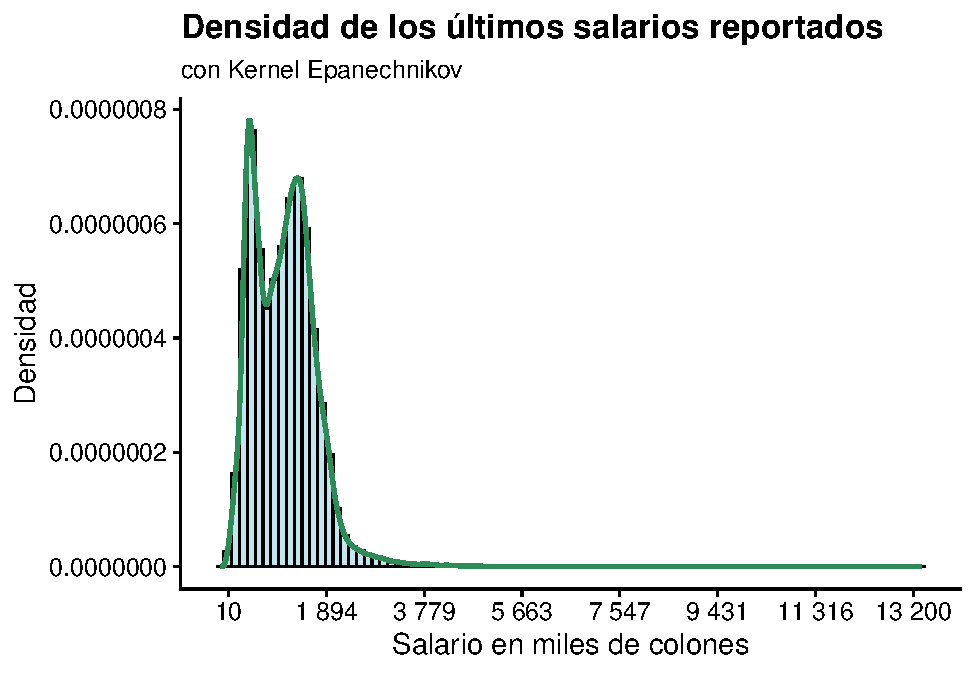
\includegraphics{Tarea1_files/figure-latex/unnamed-chunk-12-1.pdf}

\hypertarget{densidad-de-los-salarios-por-kernel-no-paramuxe9trica}{%
\subsection{Densidad de los salarios por kernel (no
paramétrica)}\label{densidad-de-los-salarios-por-kernel-no-paramuxe9trica}}

Una forma de aproximar la densidad de una muestra es mediante el uso de
kernels. Existen diversos tipos de kernels, como el kernel normal,
kernel epanechnikov, kernel triangular, kernel coseno y kernel
rectangular. A continuación, se presentan los gráficos de la densidad de
los salarios utilizando cada uno de estos tipos de kernels mediante la
función Density en el programa R.

\hypertarget{densidad-de-los-salarios-por-kernel-usando-como-kernel-biweigth}{%
\subsubsection{Densidad de los salarios por kernel usando como kernel
Biweigth}\label{densidad-de-los-salarios-por-kernel-usando-como-kernel-biweigth}}

\begin{Shaded}
\begin{Highlighting}[]
\NormalTok{density\_biweight }\OtherTok{\textless{}{-}} \FunctionTok{density}\NormalTok{(base\_salarios}\SpecialCharTok{$}\NormalTok{Ultimo.Salario, }\AttributeTok{kernel =} \StringTok{"biweight"}\NormalTok{)}
\end{Highlighting}
\end{Shaded}

\begin{Shaded}
\begin{Highlighting}[]
\NormalTok{grafBase }\OtherTok{\textless{}{-}}\NormalTok{ grafBase }\SpecialCharTok{+}
  \FunctionTok{geom\_line}\NormalTok{(}\AttributeTok{data =} \FunctionTok{data.frame}\NormalTok{(}\AttributeTok{x =}\NormalTok{ density\_biweight}\SpecialCharTok{$}\NormalTok{x, }\AttributeTok{y =}\NormalTok{ density\_biweight}\SpecialCharTok{$}\NormalTok{y),}
            \FunctionTok{aes}\NormalTok{(x, y), }\AttributeTok{color =} \StringTok{"cyan4"}\NormalTok{, }\AttributeTok{size =} \DecValTok{1}\NormalTok{) }\SpecialCharTok{+}  
  \FunctionTok{labs}\NormalTok{(}\AttributeTok{title =} \StringTok{"Densidad de los últimos salarios reportados "}\NormalTok{, }
       \AttributeTok{subtitle =} \StringTok{"con Kernel Biweight"}\NormalTok{, }\AttributeTok{x =} \StringTok{"Salario en miles de colones"}\NormalTok{, }\AttributeTok{y =} \StringTok{"Densidad"}\NormalTok{)}
\end{Highlighting}
\end{Shaded}

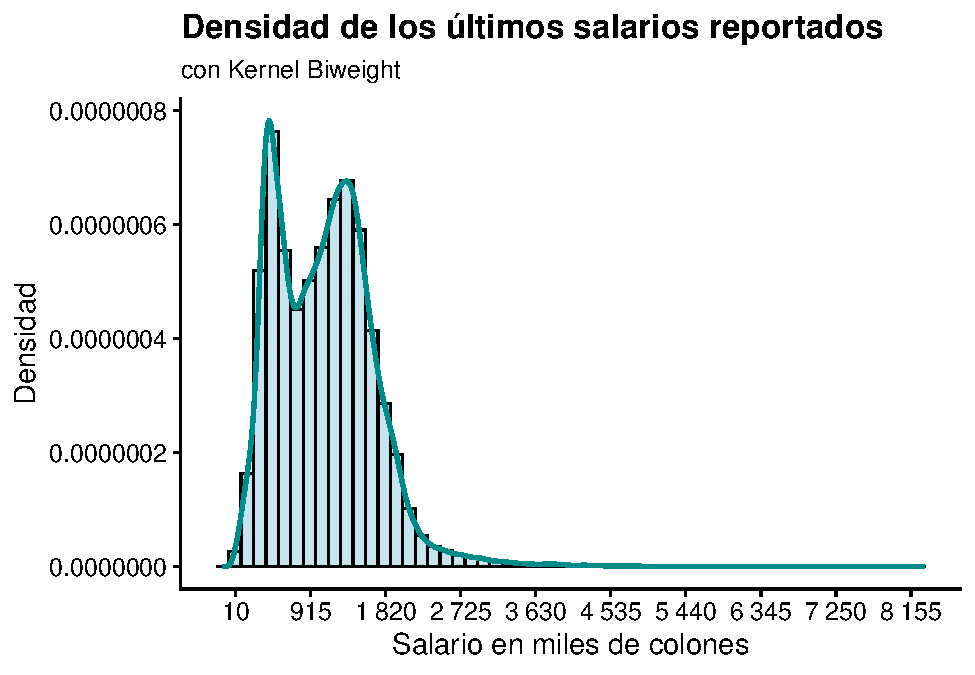
\includegraphics{Tarea1_files/figure-latex/unnamed-chunk-15-1.pdf}

\hypertarget{densidad-de-los-salarios-por-kernel-usando-como-kernel-normal}{%
\subsubsection{Densidad de los salarios por kernel usando como kernel
Normal}\label{densidad-de-los-salarios-por-kernel-usando-como-kernel-normal}}

\begin{Shaded}
\begin{Highlighting}[]
\NormalTok{density\_normal }\OtherTok{\textless{}{-}} \FunctionTok{density}\NormalTok{(base\_salarios}\SpecialCharTok{$}\NormalTok{Ultimo.Salario,}\AttributeTok{kernel =} \StringTok{"gaussian"}\NormalTok{)}
\end{Highlighting}
\end{Shaded}

\begin{Shaded}
\begin{Highlighting}[]
\NormalTok{grafBase }\OtherTok{\textless{}{-}}\NormalTok{ grafBase }\SpecialCharTok{+}
  \FunctionTok{geom\_line}\NormalTok{(}\AttributeTok{data =} \FunctionTok{data.frame}\NormalTok{(}\AttributeTok{x =}\NormalTok{ density\_normal}\SpecialCharTok{$}\NormalTok{x, }\AttributeTok{y =}\NormalTok{ density\_normal}\SpecialCharTok{$}\NormalTok{y),}
            \FunctionTok{aes}\NormalTok{(x, y), }\AttributeTok{color =} \StringTok{"red3"}\NormalTok{, }\AttributeTok{size =} \DecValTok{1}\NormalTok{) }\SpecialCharTok{+}  
  \FunctionTok{labs}\NormalTok{(}\AttributeTok{title =} \StringTok{"Densidad de los últimos salarios reportados "}\NormalTok{, }
       \AttributeTok{subtitle =} \StringTok{"con Kernel Normal"}\NormalTok{, }\AttributeTok{x =} \StringTok{"Salario en miles de colones"}\NormalTok{, }\AttributeTok{y =} \StringTok{"Densidad"}\NormalTok{)}
\end{Highlighting}
\end{Shaded}

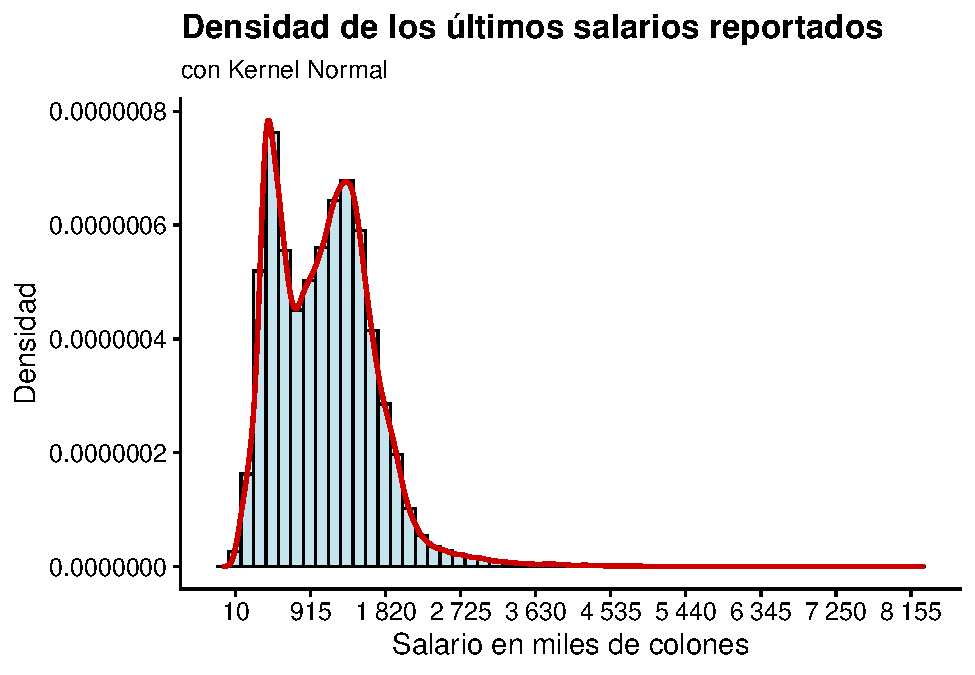
\includegraphics{Tarea1_files/figure-latex/unnamed-chunk-18-1.pdf}

\hypertarget{densidad-de-los-salarios-por-kernel-usando-como-kernel-epanechnikov}{%
\subsubsection{Densidad de los salarios por kernel usando como kernel
Epanechnikov}\label{densidad-de-los-salarios-por-kernel-usando-como-kernel-epanechnikov}}

\begin{Shaded}
\begin{Highlighting}[]
\NormalTok{density\_epanechnikov }\OtherTok{\textless{}{-}} \FunctionTok{density}\NormalTok{(base\_salarios}\SpecialCharTok{$}\NormalTok{Ultimo.Salario,}\AttributeTok{kernel =} \StringTok{"epanechnikov"}\NormalTok{)}
\end{Highlighting}
\end{Shaded}

\begin{Shaded}
\begin{Highlighting}[]
\NormalTok{grafBase }\OtherTok{\textless{}{-}}\NormalTok{ grafBase }\SpecialCharTok{+}
  \FunctionTok{geom\_line}\NormalTok{(}\AttributeTok{data =} \FunctionTok{data.frame}\NormalTok{(}\AttributeTok{x =}\NormalTok{ density\_epanechnikov}\SpecialCharTok{$}\NormalTok{x, }\AttributeTok{y =}\NormalTok{ density\_epanechnikov}\SpecialCharTok{$}\NormalTok{y),}
            \FunctionTok{aes}\NormalTok{(x, y), }\AttributeTok{color =} \StringTok{"seagreen"}\NormalTok{, }\AttributeTok{size =} \DecValTok{1}\NormalTok{) }\SpecialCharTok{+}  
  \FunctionTok{labs}\NormalTok{(}\AttributeTok{title =} \StringTok{"Densidad de los últimos salarios reportados "}\NormalTok{,}
       \AttributeTok{subtitle =} \StringTok{"con Kernel Epanechnikov"}\NormalTok{, }\AttributeTok{x =} \StringTok{"Salario en miles de colones"}\NormalTok{, }\AttributeTok{y =} \StringTok{"Densidad"}\NormalTok{)}
\end{Highlighting}
\end{Shaded}

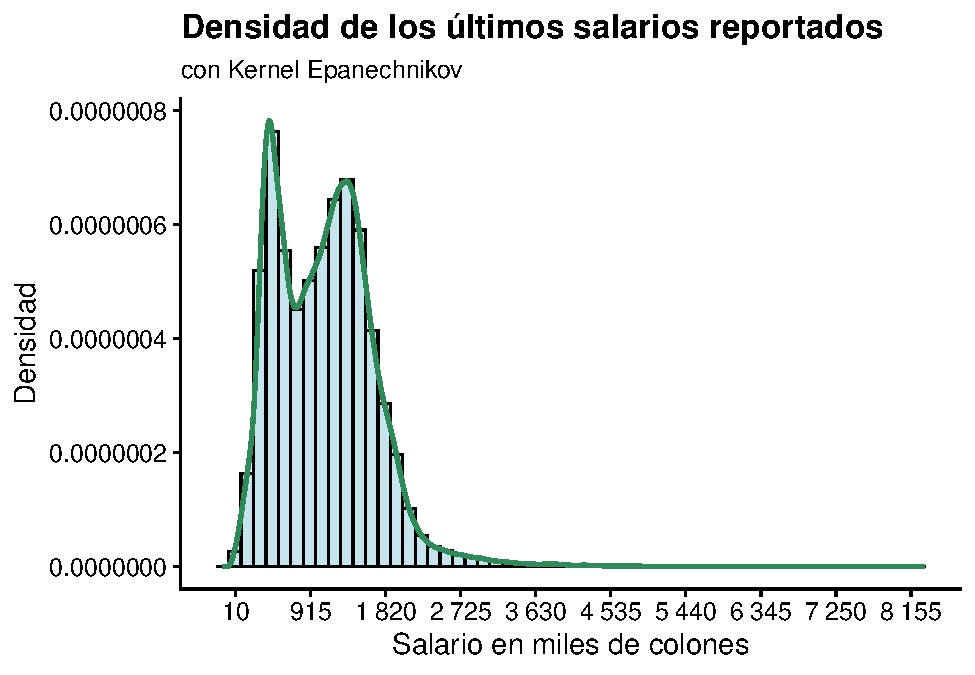
\includegraphics{Tarea1_files/figure-latex/unnamed-chunk-21-1.pdf}

\hypertarget{densidad-de-los-salarios-por-kernel-usando-como-kernel-coseno}{%
\subsubsection{Densidad de los salarios por kernel usando como kernel
Coseno}\label{densidad-de-los-salarios-por-kernel-usando-como-kernel-coseno}}

\begin{Shaded}
\begin{Highlighting}[]
\NormalTok{density\_coseno }\OtherTok{\textless{}{-}} \FunctionTok{density}\NormalTok{(base\_salarios}\SpecialCharTok{$}\NormalTok{Ultimo.Salario,}\AttributeTok{kernel =} \StringTok{"cosine"}\NormalTok{)}
\end{Highlighting}
\end{Shaded}

\begin{Shaded}
\begin{Highlighting}[]
\NormalTok{grafBase }\OtherTok{\textless{}{-}}\NormalTok{ grafBase }\SpecialCharTok{+}
  \FunctionTok{geom\_line}\NormalTok{(}\AttributeTok{data =} \FunctionTok{data.frame}\NormalTok{(}\AttributeTok{x =}\NormalTok{ density\_coseno}\SpecialCharTok{$}\NormalTok{x, }\AttributeTok{y =}\NormalTok{ density\_coseno}\SpecialCharTok{$}\NormalTok{y),}
            \FunctionTok{aes}\NormalTok{(x, y), }\AttributeTok{color =} \StringTok{"hotpink1"}\NormalTok{, }\AttributeTok{size =} \DecValTok{1}\NormalTok{) }\SpecialCharTok{+}  
  \FunctionTok{labs}\NormalTok{(}\AttributeTok{title =} \StringTok{"Densidad de los últimos salarios reportados "}\NormalTok{,}
       \AttributeTok{subtitle =} \StringTok{"con Kernel Coseno"}\NormalTok{, }\AttributeTok{x =} \StringTok{"Salario en miles de colones"}\NormalTok{, }\AttributeTok{y =} \StringTok{"Densidad"}\NormalTok{)}
\end{Highlighting}
\end{Shaded}

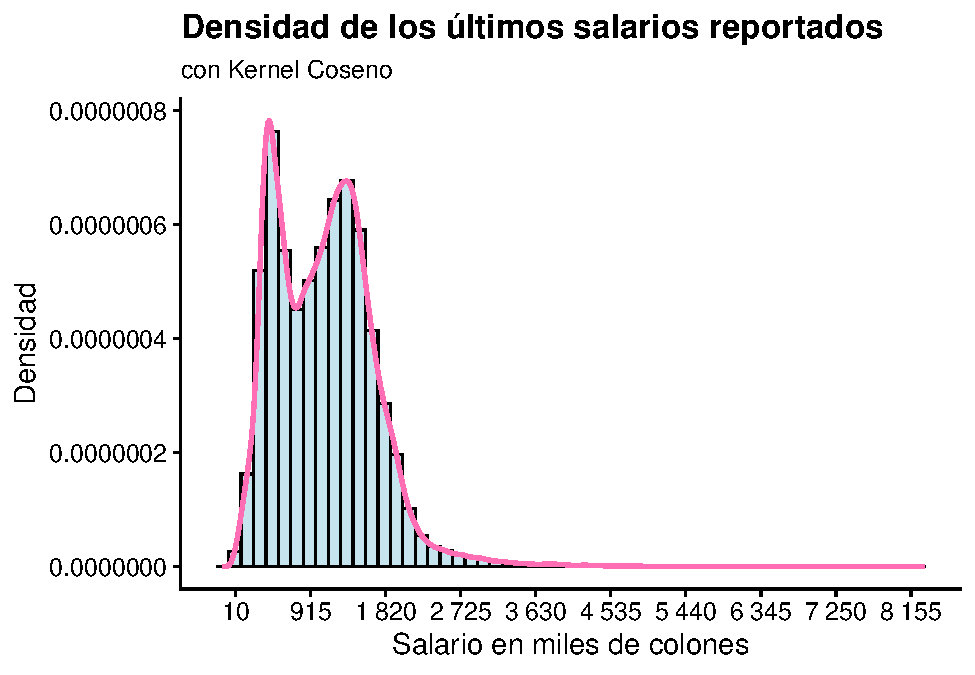
\includegraphics{Tarea1_files/figure-latex/unnamed-chunk-24-1.pdf}

\hypertarget{densidad-de-los-salarios-por-kernel-usando-como-kernel-rectangular}{%
\subsubsection{Densidad de los salarios por kernel usando como kernel
Rectangular}\label{densidad-de-los-salarios-por-kernel-usando-como-kernel-rectangular}}

\begin{Shaded}
\begin{Highlighting}[]
\NormalTok{density\_rectangular }\OtherTok{\textless{}{-}} \FunctionTok{density}\NormalTok{(base\_salarios}\SpecialCharTok{$}\NormalTok{Ultimo.Salario,}\AttributeTok{kernel =} \StringTok{"rectangular"}\NormalTok{)}
\end{Highlighting}
\end{Shaded}

\begin{Shaded}
\begin{Highlighting}[]
\NormalTok{grafBase }\OtherTok{\textless{}{-}}\NormalTok{ grafBase }\SpecialCharTok{+}
  \FunctionTok{geom\_line}\NormalTok{(}\AttributeTok{data =} \FunctionTok{data.frame}\NormalTok{(}\AttributeTok{x =}\NormalTok{ density\_rectangular}\SpecialCharTok{$}\NormalTok{x, }\AttributeTok{y =}\NormalTok{ density\_rectangular}\SpecialCharTok{$}\NormalTok{y),}
            \FunctionTok{aes}\NormalTok{(x, y), }\AttributeTok{color =} \StringTok{"goldenrod2"}\NormalTok{, }\AttributeTok{size =} \DecValTok{1}\NormalTok{) }\SpecialCharTok{+}  
  \FunctionTok{labs}\NormalTok{(}\AttributeTok{title =} \StringTok{"Densidad de los últimos salarios reportados "}\NormalTok{,}
       
       \AttributeTok{subtitle =} \StringTok{"con Kernel Rectangular"}\NormalTok{, }\AttributeTok{x =} \StringTok{"Salario en miles de colones"}\NormalTok{, }\AttributeTok{y =} \StringTok{"Densidad"}\NormalTok{)}
\end{Highlighting}
\end{Shaded}

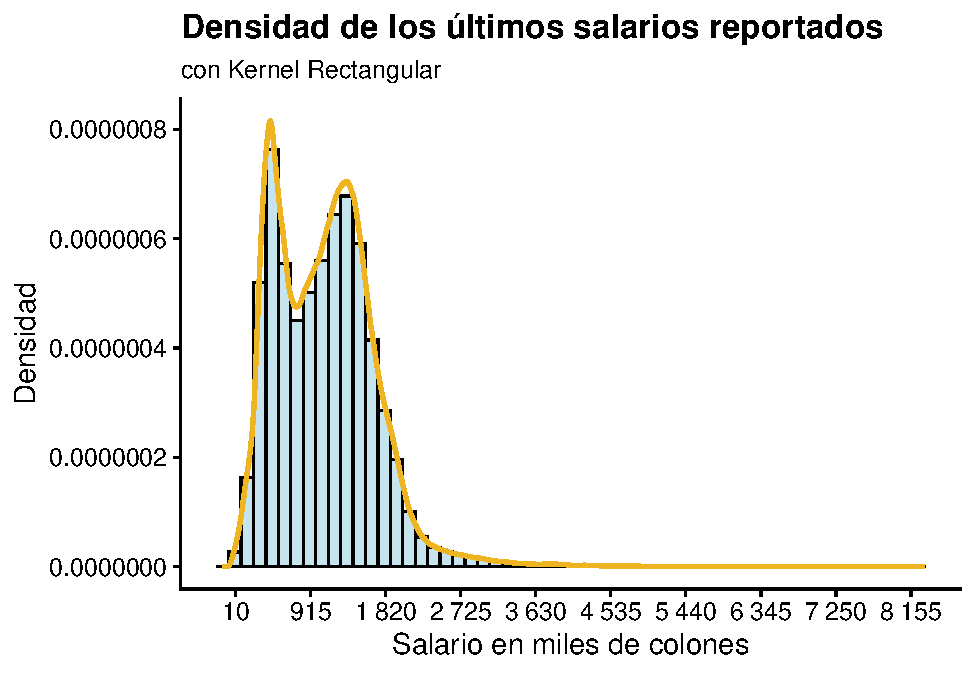
\includegraphics{Tarea1_files/figure-latex/unnamed-chunk-27-1.pdf}

\hypertarget{densidad-de-los-salarios-con-todos-los-kernel}{%
\subsubsection{Densidad de los salarios con todos los
kernel}\label{densidad-de-los-salarios-con-todos-los-kernel}}

En el siguiente gráfico, se colocó todos los kernel en un sólo gráfico.
En este gráfico lo que se puede observar es que la gráfica de kernel
epanechnikov es la que más se distancia del resto de las gráficas.

\begin{Shaded}
\begin{Highlighting}[]
\FunctionTok{ggplot}\NormalTok{(base\_salarios, }\FunctionTok{aes}\NormalTok{(}\AttributeTok{x =}\NormalTok{ Ultimo.Salario)) }\SpecialCharTok{+}
  \FunctionTok{geom\_histogram}\NormalTok{(}\AttributeTok{binwidth =} \DecValTok{150000}\NormalTok{, }\AttributeTok{fill =} \StringTok{"lightblue"}\NormalTok{, }\AttributeTok{color =} \StringTok{"black"}\NormalTok{, }\AttributeTok{alpha =} \FloatTok{0.7}\NormalTok{, }
                 \FunctionTok{aes}\NormalTok{(}\AttributeTok{y =}\NormalTok{ ..density..)) }\SpecialCharTok{+}
  \FunctionTok{geom\_line}\NormalTok{(}\AttributeTok{data =} \FunctionTok{data.frame}\NormalTok{(}\AttributeTok{x =}\NormalTok{ density\_normal}\SpecialCharTok{$}\NormalTok{x, }\AttributeTok{y =}\NormalTok{ density\_normal}\SpecialCharTok{$}\NormalTok{y),}
            \FunctionTok{aes}\NormalTok{(x, y, }\AttributeTok{color =} \StringTok{"Normal"}\NormalTok{), }\AttributeTok{size =} \DecValTok{2}\NormalTok{) }\SpecialCharTok{+}
  \FunctionTok{geom\_line}\NormalTok{(}\AttributeTok{data =} \FunctionTok{data.frame}\NormalTok{(}\AttributeTok{x =}\NormalTok{ density\_biweight}\SpecialCharTok{$}\NormalTok{x, }\AttributeTok{y =}\NormalTok{ density\_biweight}\SpecialCharTok{$}\NormalTok{y),}
            \FunctionTok{aes}\NormalTok{(x, y, }\AttributeTok{color =} \StringTok{"Biweight"}\NormalTok{), }\AttributeTok{size =} \FloatTok{1.7}\NormalTok{) }\SpecialCharTok{+}
  \FunctionTok{geom\_line}\NormalTok{(}\AttributeTok{data =} \FunctionTok{data.frame}\NormalTok{(}\AttributeTok{x =}\NormalTok{ density\_coseno}\SpecialCharTok{$}\NormalTok{x, }\AttributeTok{y =}\NormalTok{ density\_coseno}\SpecialCharTok{$}\NormalTok{y),}
            \FunctionTok{aes}\NormalTok{(x, y, }\AttributeTok{color =} \StringTok{"Coseno"}\NormalTok{), }\AttributeTok{size =} \FloatTok{1.4}\NormalTok{) }\SpecialCharTok{+}
  \FunctionTok{geom\_line}\NormalTok{(}\AttributeTok{data =} \FunctionTok{data.frame}\NormalTok{(}\AttributeTok{x =}\NormalTok{ density\_rectangular}\SpecialCharTok{$}\NormalTok{x, }\AttributeTok{y =}\NormalTok{ density\_rectangular}\SpecialCharTok{$}\NormalTok{y),}
            \FunctionTok{aes}\NormalTok{(x, y, }\AttributeTok{color =} \StringTok{"Rectangular"}\NormalTok{), }\AttributeTok{size =} \FloatTok{1.1}\NormalTok{) }\SpecialCharTok{+}
  \FunctionTok{geom\_line}\NormalTok{(}\AttributeTok{data =} \FunctionTok{data.frame}\NormalTok{(}\AttributeTok{x =}\NormalTok{ density\_epanechnikov}\SpecialCharTok{$}\NormalTok{x, }\AttributeTok{y =}\NormalTok{ density\_epanechnikov}\SpecialCharTok{$}\NormalTok{y),}
            \FunctionTok{aes}\NormalTok{(x, y, }\AttributeTok{color =} \StringTok{"Epanechnikov"}\NormalTok{), }\AttributeTok{size =} \FloatTok{0.8}\NormalTok{) }\SpecialCharTok{+}
  \FunctionTok{labs}\NormalTok{(}\AttributeTok{title =} \StringTok{"Densidad de los últimos salarios reportados"}\NormalTok{, }
       \AttributeTok{x =} \StringTok{"Salario en miles de colones"}\NormalTok{, }\AttributeTok{y =} \StringTok{"Densidad"}\NormalTok{) }\SpecialCharTok{+}
  \FunctionTok{theme\_cowplot}\NormalTok{() }\SpecialCharTok{+}
  \FunctionTok{scale\_x\_continuous}\NormalTok{(}
    \AttributeTok{breaks =} \FunctionTok{seq}\NormalTok{(}\FunctionTok{min}\NormalTok{(base\_salarios}\SpecialCharTok{$}\NormalTok{Ultimo.Salario), }\FunctionTok{max}\NormalTok{(base\_salarios}\SpecialCharTok{$}\NormalTok{Ultimo.Salario), }
                 \AttributeTok{length.out =} \DecValTok{10}\NormalTok{),}
    \AttributeTok{labels =}\NormalTok{ scales}\SpecialCharTok{::}\FunctionTok{label\_number}\NormalTok{(}\AttributeTok{big.mark =} \StringTok{" "}\NormalTok{, }\AttributeTok{decimal.mark =} \StringTok{"."}\NormalTok{, }\AttributeTok{scale =} \FloatTok{1e{-}3}\NormalTok{)}
\NormalTok{  ) }\SpecialCharTok{+}
  \FunctionTok{scale\_color\_manual}\NormalTok{(}\AttributeTok{values =} \FunctionTok{c}\NormalTok{(}\StringTok{"red3"}\NormalTok{, }\StringTok{"cyan4"}\NormalTok{, }\StringTok{"hotpink1"}\NormalTok{, }\StringTok{"goldenrod2"}\NormalTok{, }\StringTok{"seagreen"}\NormalTok{),}
                     \AttributeTok{name =} \StringTok{"Kernel"}\NormalTok{,}
                     \AttributeTok{labels =} \FunctionTok{c}\NormalTok{(}\StringTok{"Normal"}\NormalTok{, }\StringTok{"Biweight"}\NormalTok{, }\StringTok{"Coseno"}\NormalTok{, }\StringTok{"Rectangular"}\NormalTok{, }
                                \StringTok{"Epanechnikov"}\NormalTok{)) }\SpecialCharTok{+}
  \FunctionTok{theme}\NormalTok{(}\AttributeTok{legend.text =} \FunctionTok{element\_text}\NormalTok{(}\AttributeTok{size =} \DecValTok{6}\NormalTok{),}
        \AttributeTok{legend.title =} \FunctionTok{element\_text}\NormalTok{(}\AttributeTok{size =} \DecValTok{9}\NormalTok{))}
\end{Highlighting}
\end{Shaded}

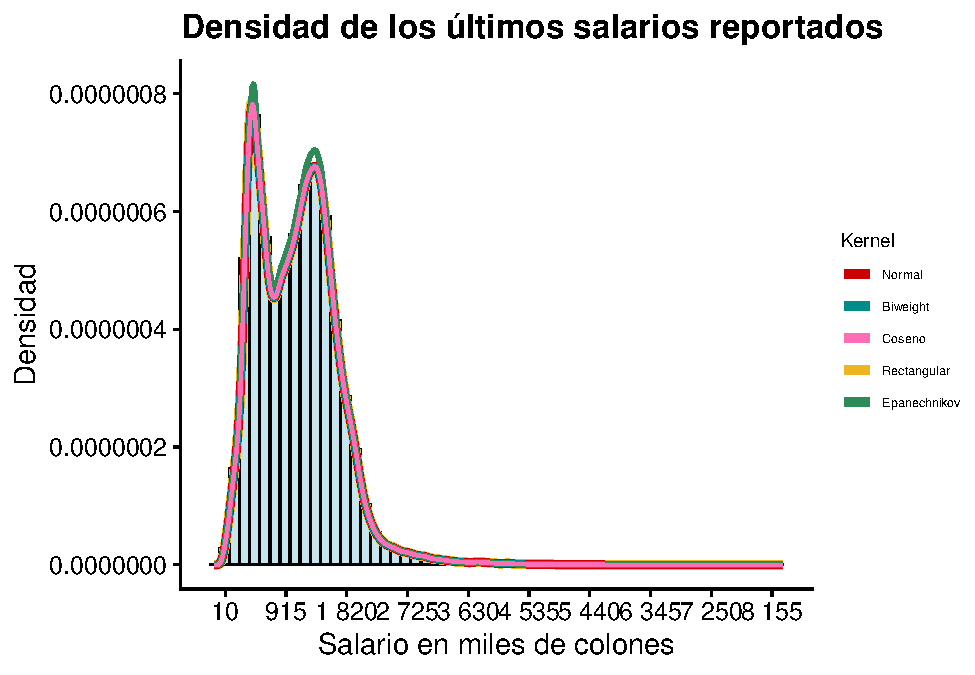
\includegraphics{Tarea1_files/figure-latex/unnamed-chunk-28-1.pdf}

\hypertarget{parte-iii}{%
\section{Parte III}\label{parte-iii}}

El Criterio de Información de Akaike (AIC) es una medida utilizada en
estadísticas y modelado para comparar modelos estadísticos.El AIC se
calcula utilizando la siguiente fórmula:

\[ AIC= 2*N−2*log(L) \]

Donde \[L\] representa la funcion de máxima verosimilitud del modelo y
\[N\] representa el número de parámetros en el modelo. El modelo
penaliza aquellos modelos que utilizan varios parámetros, ya que se
busca el modelo con mayor simpleza. Cuando se comparan varios modelos,
el modelo con el AIC más bajo se considera preferido.

\hypertarget{anuxe1lisis-del-aic-de-la-variable-ultimo.salario-mediante-la-funciuxf3n-model_select}{%
\subsection{Análisis del AIC de la variable Ultimo.Salario mediante la
función
model\_select}\label{anuxe1lisis-del-aic-de-la-variable-ultimo.salario-mediante-la-funciuxf3n-model_select}}

\begin{Shaded}
\begin{Highlighting}[]
\FunctionTok{model\_select}\NormalTok{(base\_salarios}\SpecialCharTok{$}\NormalTok{Ultimo.Salario)}
\end{Highlighting}
\end{Shaded}

\begin{verbatim}
## Maximum likelihood estimates for the Skew Student-t model 
##        mean           sd           nu           xi  
## 1064002.056   617965.176       53.872        2.401
\end{verbatim}

Vemos que la funcion model select del paquete univariateML sugiere una
distribución t-student para representar los datos de Ultimo.Salario.

\hypertarget{anuxe1lisis-del-aic-de-la-variable-ultimo.salario-mediante-la-funciuxf3n-fit.cont}{%
\subsection{Análisis del AIC de la variable Ultimo.Salario mediante la
función
fit.cont}\label{anuxe1lisis-del-aic-de-la-variable-ultimo.salario-mediante-la-funciuxf3n-fit.cont}}

\begin{Shaded}
\begin{Highlighting}[]
\FunctionTok{fit.cont}\NormalTok{(base\_salarios}\SpecialCharTok{$}\NormalTok{Ultimo.Salario)}
\end{Highlighting}
\end{Shaded}

\begin{longtable}[]{@{}ll@{}}
\toprule\noalign{}
Distribución & AIC \\
\midrule\noalign{}
\endhead
\bottomrule\noalign{}
\endlastfoot
Cauchy & 3 158 816.91 \\
Uniforme & NULL \\
Lognormal & 3 119 863.45 \\
Weibull & 3 104 610.52 \\
F & 3 705 605.8 \\
Student & 3 850 227.82 \\
\end{longtable}

Bajo el criterio de AIC, el modelo con el valor más bajo es el Weibull,
seguido por el Lognormal con una diferencia de 115 252.93 unidades. En
comparación, la diferencia entre el Weibull y la distribución t que fue
la que el fit.cont() recomendaba, es de 745 617.3 unidades. Es por este
motivo, que al comparar ambos resultados, se opta por el modelo Weibull
para representar los salarios.

\hypertarget{construcciuxf3n-de-un-intervalo-de-confianza-para-la-media-y-la-desviaciuxf3n-estuxe1ndar-usando-la-funciuxf3n-bootstrapml}{%
\subsection{Construcción de un intervalo de confianza para la media y la
desviación estándar usando la función
bootstrapml}\label{construcciuxf3n-de-un-intervalo-de-confianza-para-la-media-y-la-desviaciuxf3n-estuxe1ndar-usando-la-funciuxf3n-bootstrapml}}

\begin{Shaded}
\begin{Highlighting}[]
\CommentTok{\#Creamos un objeto de distribución}
\NormalTok{distribucionml }\OtherTok{\textless{}{-}} \FunctionTok{mlweibull}\NormalTok{(base\_salarios}\SpecialCharTok{$}\NormalTok{Ultimo.Salario)}

\FunctionTok{bootstrapml}\NormalTok{(distribucionml, }
            \AttributeTok{map =} \ControlFlowTok{function}\NormalTok{(x) }\FunctionTok{mean}\NormalTok{(x))}
\end{Highlighting}
\end{Shaded}

\begin{verbatim}
##     2.5%    97.5% 
## 606971.1 610993.1
\end{verbatim}

Es decir, con una confianza del 95\%, al aplicar bootstrapml, se estima
que la media de la distribución Weibull, está entre los 606 922.4
colones y los 611 076.8 colones.

\begin{Shaded}
\begin{Highlighting}[]
\FunctionTok{bootstrapml}\NormalTok{(distribucionml, }
            \AttributeTok{map =} \ControlFlowTok{function}\NormalTok{(x) }\FunctionTok{sd}\NormalTok{(x))}
\end{Highlighting}
\end{Shaded}

\begin{verbatim}
##     2.5%    97.5% 
## 858230.8 864269.3
\end{verbatim}

Por su parte, la desviación estándar de la distribución Weibull al
aplicar el bootstrapml está entre 858 674.9 y 864 239.7.

\hypertarget{parte-iv}{%
\section{Parte IV}\label{parte-iv}}

\hypertarget{estimaciuxf3n-de-la-densidad-del-kernel}{%
\subsection{Estimación de la densidad del
kernel}\label{estimaciuxf3n-de-la-densidad-del-kernel}}

La función kde(Kernel Density Estimation) del paquete ks en R,c omo su
nombre indica, lleva a cabo una estimación no paramétrica de la densidad
de kernel para datos de 1 hasta 6 dimensiones. Esta función se utiliza
comúnmente cuando la función de distribución de los datos es irregular,
ya que, kde() genera una función suavizada de la misma.

\begin{Shaded}
\begin{Highlighting}[]
\FunctionTok{plot}\NormalTok{(}\FunctionTok{kde}\NormalTok{(base\_salarios}\SpecialCharTok{$}\NormalTok{Ultimo.Salario),  }\AttributeTok{main =} \StringTok{"Densidad de Kernel para los Salarios"}\NormalTok{, }\AttributeTok{xlab =} \StringTok{"Monto del Salario"}\NormalTok{, }\AttributeTok{ylab=} \StringTok{"Función de Densidad"}\NormalTok{, }\AttributeTok{col =} \StringTok{"cyan4"}\NormalTok{, }\AttributeTok{lwd =} \DecValTok{2}\NormalTok{, }\AttributeTok{las =} \DecValTok{1}\NormalTok{, }\AttributeTok{cex.axis=}\FloatTok{0.5}\NormalTok{, }\AttributeTok{cex.lab =} \FloatTok{0.8}\NormalTok{)}
\end{Highlighting}
\end{Shaded}

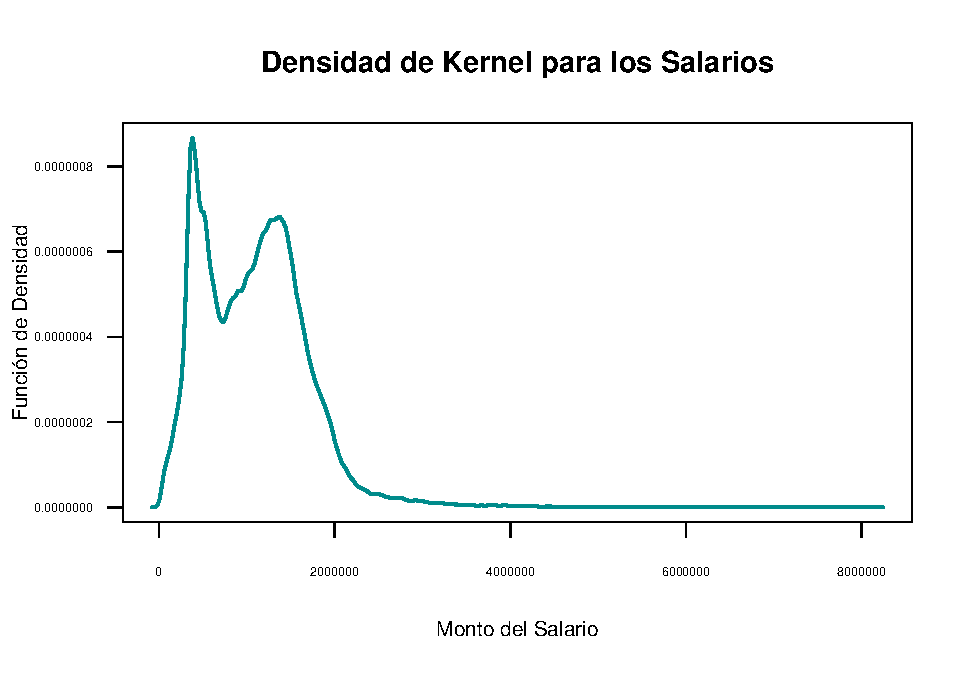
\includegraphics{Tarea1_files/figure-latex/unnamed-chunk-35-1.pdf}

\hypertarget{intervalos-de-confianza-con-bootstrap}{%
\subsection{Intervalos de confianza con
bootstrap}\label{intervalos-de-confianza-con-bootstrap}}

La función boot.ci del paquete boot en R se utiliza para calcular los
intervalos de confianza de un estadístico determinado, para lo cual la
función realiza un remuestreo bootstrap del estadístico con la muestra
de datos proporcionada. Esta función calcula los intervalos de confianza
mediante 4 métodos diferentes de bootstrap: básico, `studentized', de
percentiles y de percentiles ajustados.

\hypertarget{bootstrap-de-la-media-de-los-salarios}{%
\subsection{Bootstrap de la media de los
salarios}\label{bootstrap-de-la-media-de-los-salarios}}

\hypertarget{estimaciuxf3n-de-la-media-del-bootstrap}{%
\subsubsection{Estimación de la media del
Bootstrap}\label{estimaciuxf3n-de-la-media-del-bootstrap}}

En este caso, se consideran 1000 muestras bootstrap y se calcula la
media para cada una de las muestras.

\begin{Shaded}
\begin{Highlighting}[]
\FunctionTok{set.seed}\NormalTok{(}\DecValTok{123}\NormalTok{) }\CommentTok{\#  generar números aleatorios}

\NormalTok{bootstrap }\OtherTok{\textless{}{-}} \FunctionTok{boot}\NormalTok{(}\AttributeTok{data =}\NormalTok{ base\_salarios}\SpecialCharTok{$}\NormalTok{Ultimo.Salario, }
                  \AttributeTok{statistic =} \ControlFlowTok{function}\NormalTok{(x, indices) }\FunctionTok{mean}\NormalTok{(x[indices]), }\AttributeTok{R=}\DecValTok{1000}\NormalTok{)}
\FunctionTok{mean}\NormalTok{(bootstrap}\SpecialCharTok{$}\NormalTok{t)}
\end{Highlighting}
\end{Shaded}

\begin{verbatim}
## [1] 1080550
\end{verbatim}

\begin{Shaded}
\begin{Highlighting}[]
\NormalTok{bootstrap}\SpecialCharTok{$}\NormalTok{t0 }
\end{Highlighting}
\end{Shaded}

\begin{verbatim}
## [1] 1080558
\end{verbatim}

La media de los últimos salarios al aplicar bootstrap es de 1 080 550
colones, mientras que la media de los datos originales fue de 1 080 558.
Es decir, la diferencia entre estas es de 8 colones.

\begin{Shaded}
\begin{Highlighting}[]
\FunctionTok{boot.ci}\NormalTok{(bootstrap, }\AttributeTok{conf =} \FloatTok{0.95}\NormalTok{, }\AttributeTok{type =} \StringTok{"basic"}\NormalTok{)}
\end{Highlighting}
\end{Shaded}

\begin{verbatim}
## BOOTSTRAP CONFIDENCE INTERVAL CALCULATIONS
## Based on 1000 bootstrap replicates
## 
## CALL : 
## boot.ci(boot.out = bootstrap, conf = 0.95, type = "basic")
## 
## Intervals : 
## Level      Basic         
## 95%   (1076945, 1084276 )  
## Calculations and Intervals on Original Scale
\end{verbatim}

Con un nivel de confianza del 95\%, la media de los salarios de la base
de datos está entre 1 076 945 y 1 084 276 colones al aplicar bootstrap.

\hypertarget{histograma-de-los-resultados}{%
\subsubsection{Histograma de los
resultados}\label{histograma-de-los-resultados}}

En el siguiente histograma se presentan los resultados del Bootstrap.

\begin{Shaded}
\begin{Highlighting}[]
\FunctionTok{hist}\NormalTok{(bootstrap}\SpecialCharTok{$}\NormalTok{t, }\AttributeTok{las=}\DecValTok{1}\NormalTok{, }\AttributeTok{main=}\StringTok{"Histograma de las medias de salarios"}\NormalTok{, }\AttributeTok{xlab=}\StringTok{"Media Bootstrap"}\NormalTok{, }\AttributeTok{ylab=}\StringTok{"Frecuencia"}\NormalTok{, }\AttributeTok{col=}\StringTok{"lightblue"}\NormalTok{)}
\end{Highlighting}
\end{Shaded}

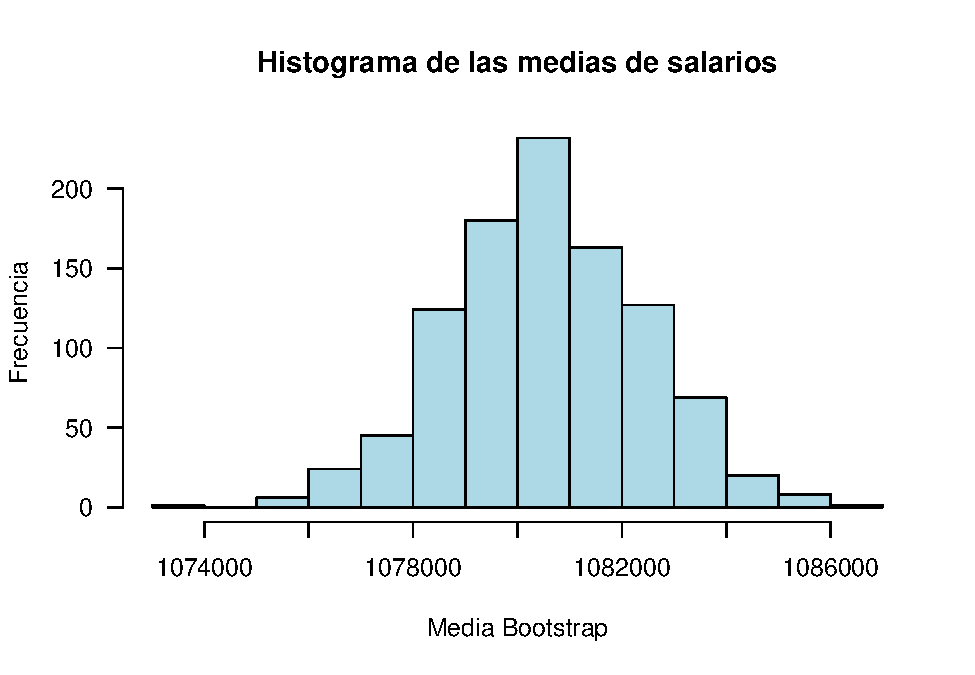
\includegraphics{Tarea1_files/figure-latex/unnamed-chunk-38-1.pdf}

\end{document}
